\documentclass{standalone}
\usepackage{tgheros}
\usepackage[utf8]{inputenc}
\usepackage[T1]{fontenc}
\usepackage{tikz}
\usetikzlibrary{shapes,matrix,positioning,fit,shapes.geometric,shapes.arrows,calc,decorations.pathreplacing,arrows.meta}
\def\roundness{0.4ex}
\tikzstyle{tiny}=[font=\fontsize{5pt}{7pt}\selectfont\sffamily]
\tikzstyle{rr}=[draw=black!66,rounded corners=\roundness,inner sep=\roundness]
\tikzstyle{arr}=[single arrow,rr,draw,tiny, text width=5em,anchor=west]
\tikzstyle{larr}=[arr,shape border rotate=180]
\tikzstyle{braceline}=[draw=black!25,decorate,decoration={brace,amplitude=1ex,mirror,raise=1ex}]
\begin{document}%
\fontsize{7pt}{9pt}\selectfont\sffamily%
\parbox{21pc}{\centering%
\begin{tikzpicture}[thick, node distance=1em,ampersand replacement=\&]
\matrix[row sep=1pt, column sep=2pt,column 1/.style={anchor=west}]{
\node[font=\bfseries] (alabel) {A.}; \\
\node[inner sep=0pt]{
\includegraphics[width=3em]{laptop1.pdf}};
\& \node[arr] {graph layout optimization};
\& \node {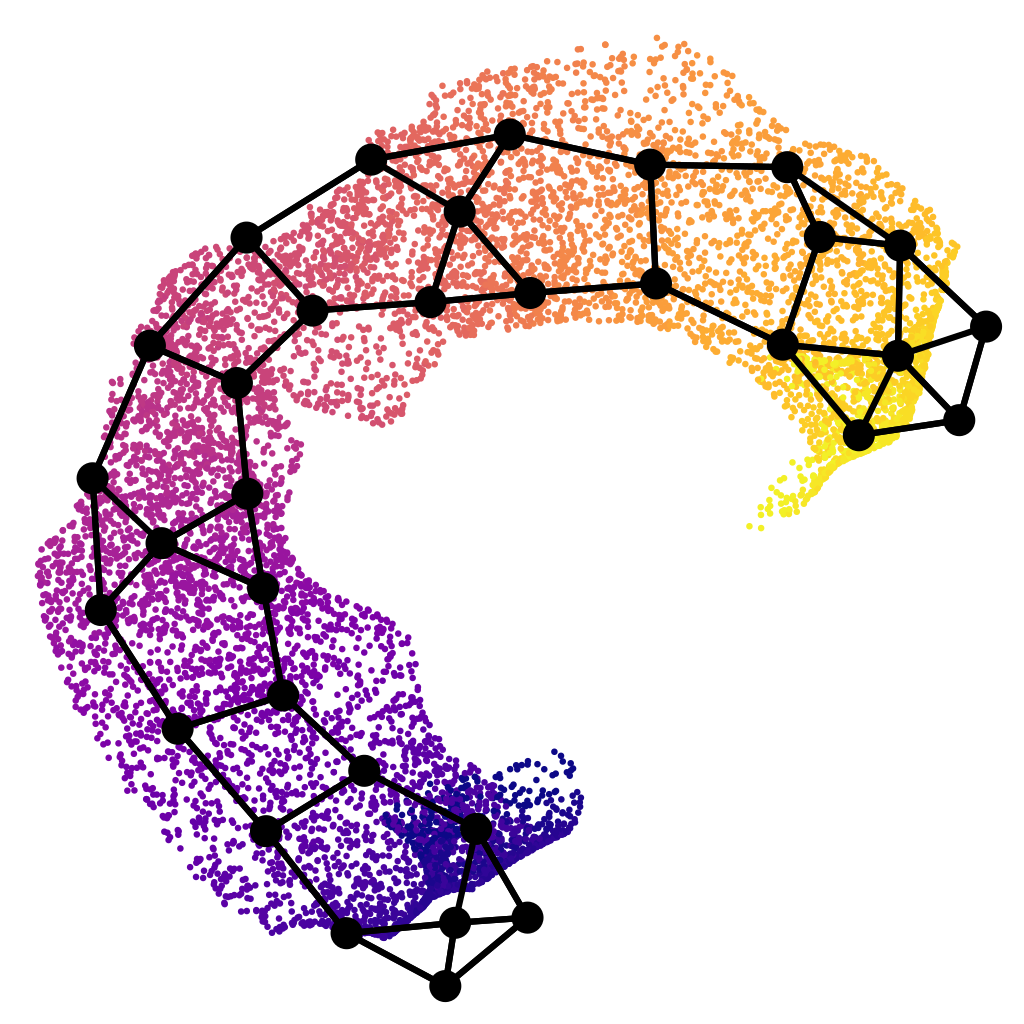
\includegraphics[height=8em]{S_graph_2d.png} };
\& \node[larr] {landmark neighborhood graph};
\& \node {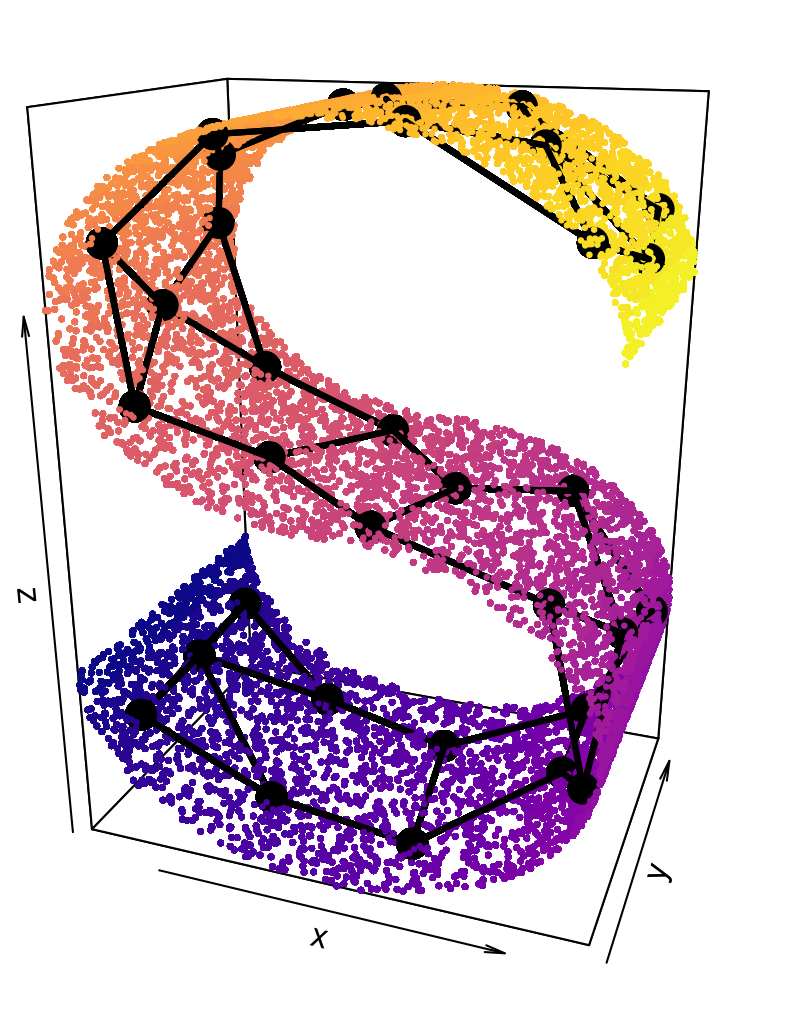
\includegraphics[height=8em]{S_graph_hd.png} };
\\
\node[font=\bfseries] (blabel) {B.}; \\
\node{
\includegraphics[width=3em]{laptop2.pdf}};
\& \node[arr] {SOM shape, level of detail};
\& \node {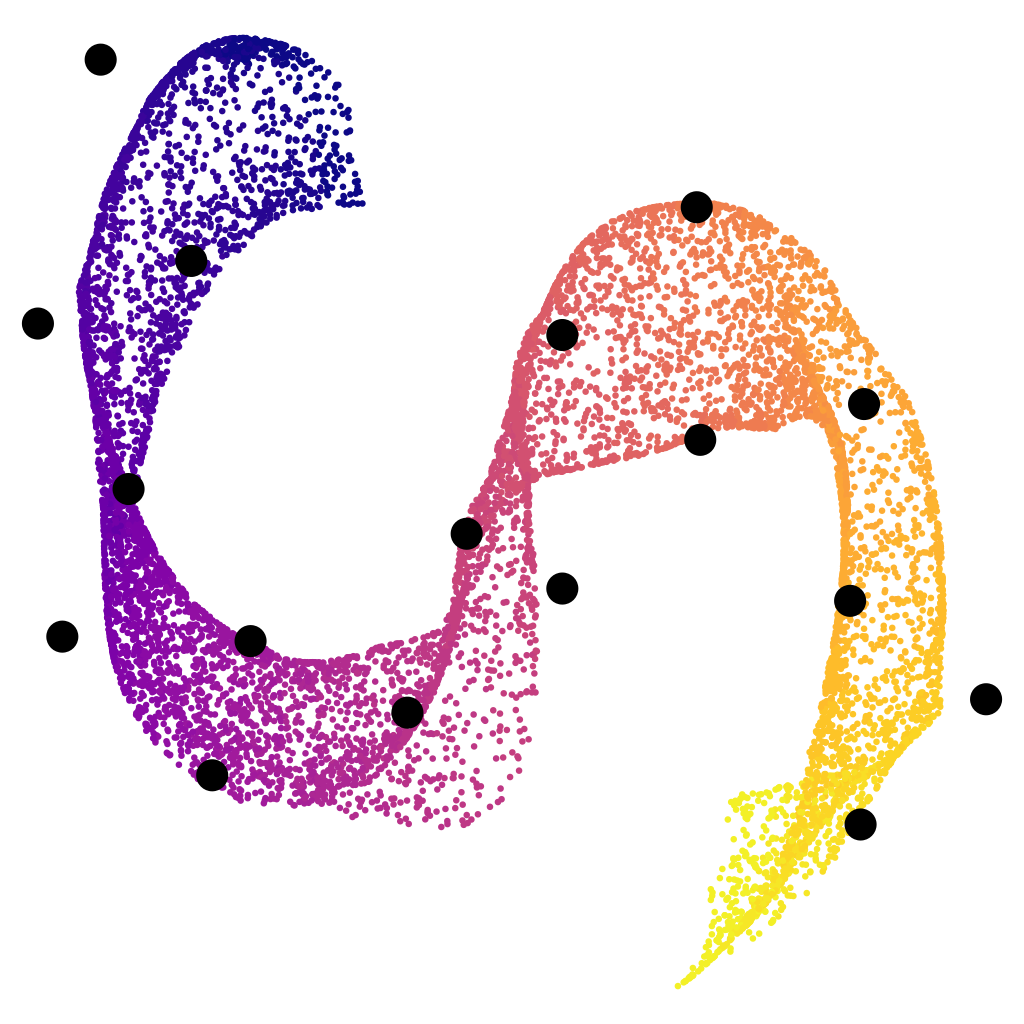
\includegraphics[height=8em]{S_som_2d.png} };
\& \node[arr] {SOM topology for training};
\& \node {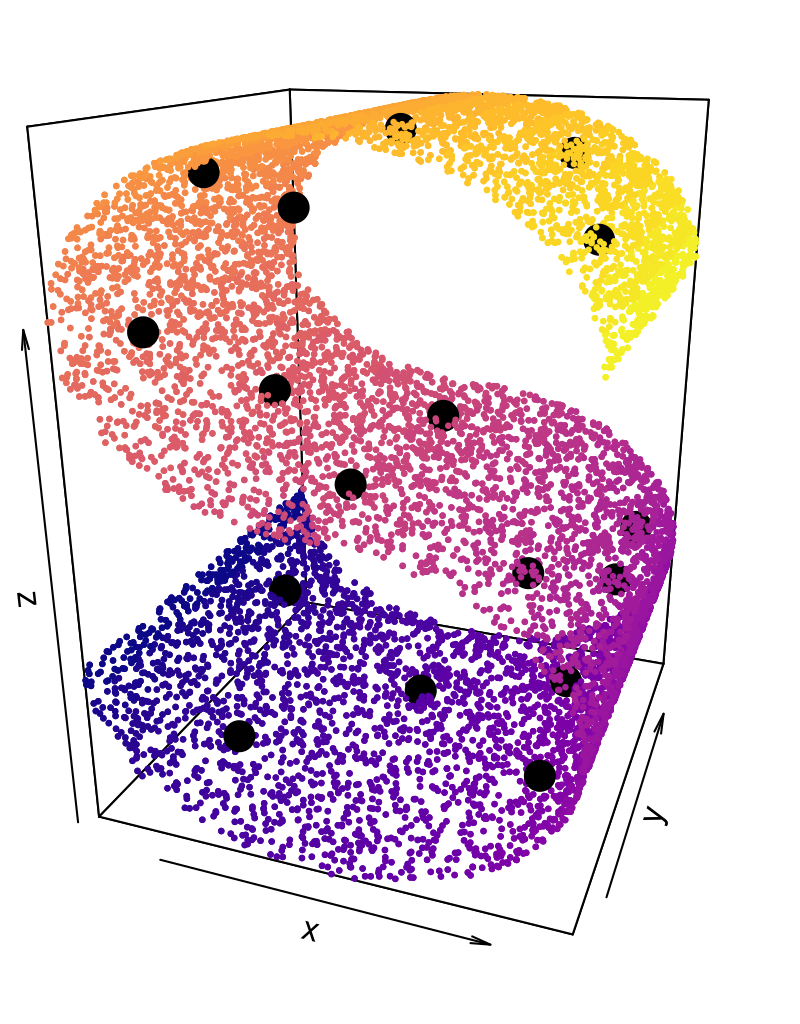
\includegraphics[height=8em]{S_som_hd.png} };
\\
};
\node[right=0 of alabel.base east,anchor=base west] {Topology reconstruction};
\node[right=0 of blabel.base east,anchor=base west] {Supervised self-organization};
\end{tikzpicture}}%
\end{document}
